\documentclass[11pt,a4paper]{article}

\usepackage[a4paper,margin=1.7cm]{geometry}
\usepackage{amsmath,amssymb,mathtools}
\usepackage{physics}
\usepackage{tikz}
\usepackage{enumitem}
\usepackage{booktabs}
\usepackage{multicol}
\usepackage{xcolor}
\usepackage{hyperref}

\hypersetup{
  colorlinks=true,
  linkcolor=blue!50!black,
  urlcolor=blue!50!black
}

\setlength{\parindent}{0pt}
\setlength{\parskip}{0.45em}
\setlist[itemize]{leftmargin=1.4em,itemsep=0.2em}
\setlist[enumerate]{leftmargin=1.6em,itemsep=0.25em}

\newcommand{\ii}{\mathrm{i}}
\newcommand{\ee}{\mathrm{e}}
\newcommand{\kB}{k_{\mathrm B}}
\newcommand{\muB}{\mu_{\mathrm B}}
\newcommand{\epsF}{\varepsilon_{\mathrm F}}
\newcommand{\TD}{T_{\mathrm D}}
\newcommand{\beff}{B_{\mathrm{eff}}}
\newcommand{\vect}[1]{\boldsymbol{#1}}

\title{\vspace{-1.2cm}B6 Cheatsheet Notes}
\author{Readable LaTeX transcription of the handwritten cheatsheet}
\date{}

\begin{document}
\maketitle

\small
This note is a readability transcription of the handwritten cheatsheet. The
derivation order and formula content have been preserved; headings and spelling
are only cleaned up where this helps reading.

\section{Crystal Definitions}

\begin{description}[leftmargin=3.2cm,style=nextline]
  \item[Lattice] An infinite set of points defined by integer sums of linearly
  independent primitive cells.

  \item[Unit cell] Any region of space that can be repeated over and over again
  to reconstruct the lattice.

  \item[Primitive unit cell] Unit cell with only one atom point.

  \item[Wigner--Seitz cell] A space that is closer to one lattice point than to
  any other lattice point.

  \item[Basis] Description of an object in a unit cell with respect to a
  reference point.

  \item[Coordination number] Number of nearest neighbours any point of the
  lattice has.

  \item[Orthorhombic lattice] Orthogonal vectors, all of different length.

  \item[Tetragonal lattice] Orthogonal vectors, two of the same length.

  \item[Reciprocal lattice] Points denoted by $\vect G$ satisfying
  \[
    \ee^{\ii \vect G \cdot \vect R}=1
    \qquad \text{for all } \vect R \text{ on the direct lattice.}
  \]

  \item[Lattice plane] Plane containing at least three non-collinear lattice
  points.

  \item[Family of lattice planes] An infinite set of equally separated parallel
  planes that contains all points of the lattice.

  \item[Brillouin zone] Unit cell in $k$-space.
\end{description}

\section{Cubic Lattices}

Here $z$ is the coordination number and $A$ is the number of atoms in the cell.

\begin{center}
\begin{tabular}{lll}
\toprule
Lattice & Coordination number $z$ & Atoms in cell $A$ \\
\midrule
SC  & $z=6$  & $A=1$ \\
BCC & $z=8$  & $A=2$ \\
FCC & $z=12$ & $A=4$ \\
\bottomrule
\end{tabular}
\end{center}

Basis points:
\[
\begin{aligned}
\text{BCC:}\quad &(0,0,0),\ \left(\frac12,\frac12,\frac12\right),\\
\text{FCC:}\quad &(0,0,0),\
\left(0,\frac12,\frac12\right),\
\left(\frac12,0,\frac12\right),\
\left(\frac12,\frac12,0\right).
\end{aligned}
\]

\section{Reciprocal Lattice and Miller Planes}

\[
\ee^{\ii \vect G\cdot \vect R}=1,
\qquad
\vect G = h\vect b_1+k\vect b_2+l\vect b_3,
\qquad
\vect R=n_1\vect a_1+n_2\vect a_2+n_3\vect a_3.
\]

\[
\vect a_i\cdot \vect b_j = 2\pi \delta_{ij}.
\]

In three dimensions,
\[
  \vect b_i =
  \frac{2\pi(\vect a_j\times\vect a_k)}
  {\vect a_i\cdot(\vect a_j\times\vect a_k)}.
\]
In two dimensions, replace $\vect a_k$ by $\vect e_z$.

For orthogonal axes,
\[
  \abs{\vect b_i}=\frac{2\pi}{\abs{\vect a_i}}.
\]

For an $(hkl)$ plane, the intercepts are
\[
  \frac{\vect a_1}{h}:\frac{\vect a_2}{k}:\frac{\vect a_3}{l}.
\]
With
\[
  \vect r_1=\frac{\vect a_1}{h}-\frac{\vect a_2}{k},
  \qquad
  \vect r_2=\frac{\vect a_2}{k}-\frac{\vect a_3}{l},
\]
one has
\[
  \vect G\cdot \vect r_1=\vect G\cdot \vect r_2=0,
\]
so $\vect G$ is perpendicular to the plane.

For adjacent planes,
\[
  \vect G\cdot \vect r = 2\pi m,
  \qquad
  \vect G\cdot(\vect r_1-\vect r_2)=2\pi.
\]
Therefore
\[
  d=\frac{2\pi}{\abs{\vect G}}.
\]

Using $\vect G=h\vect b_1+k\vect b_2+l\vect b_3$,
\[
  d=
  \frac{2\pi}{\abs{\vect G}}
  =
  \frac{2\pi}
  {\sqrt{h^2\abs{\vect b_1}^2+k^2\abs{\vect b_2}^2+l^2\abs{\vect b_3}^2}}.
\]
For a cubic lattice,
\[
  d=\frac{a}{\sqrt{h^2+k^2+l^2}}.
\]

\section{Diffraction}

\[
  \Gamma =
  \frac{2\pi}{\hbar}\,
  \delta(E_{k'}-E_k)\,
  \abs{\mel{k'}{V}{k}}^2.
\]

\[
\begin{aligned}
\mel{k'}{V}{k}
&=
\frac{1}{L^3}
\int d^3r\, V(\vect r)
\ee^{\ii(\vect k-\vect k')\cdot \vect r} \\
&=
\frac{1}{L^3}\sum_{\vect R}
\int_{\text{unit cell}} d^3r\, V(\vect r)
\ee^{-\ii\Delta\vect k\cdot \vect r}.
\end{aligned}
\]

With $V(\vect r+\vect R)=V(\vect r)$ and $\vect r=\vect r'+\vect R$,
\[
  \mel{k'}{V}{k}
  =
  \frac{1}{L^3}
  \sum_{\vect R}
  \ee^{-\ii\Delta\vect k\cdot \vect R}
  \int_{\text{cell}} d^3r'\,V(\vect r')
  \ee^{-\ii\Delta\vect k\cdot \vect r'}.
\]

If $\ee^{-\ii\Delta\vect k\cdot \vect R}\ne 1$, phases add up to zero. Thus
\[
  \ee^{\ii\Delta\vect k\cdot \vect R}=1,
  \qquad
  \boxed{\Delta\vect k=\vect G}.
\]

\subsection{Bragg and Laue}

Extra distance:
\[
  2d\sin\theta=n\lambda.
\]

\begin{center}
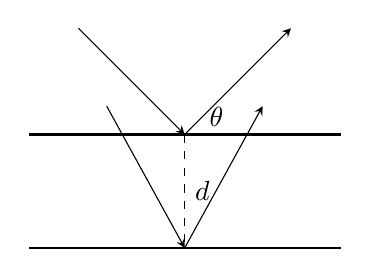
\begin{tikzpicture}[scale=0.9,>=stealth]
  \draw[thick] (-2.2,0) -- (2.2,0);
  \draw[thick] (-2.2,-1.6) -- (2.2,-1.6);
  \draw[->] (-1.5,1.5) -- (0,0);
  \draw[->] (0,0) -- (1.5,1.5);
  \draw[->] (-1.1,0.4) -- (0,-1.6);
  \draw[->] (0,-1.6) -- (1.1,0.4);
  \draw[dashed] (0,0) -- (0,-1.6);
  \node at (0.25,-0.8) {$d$};
  \node at (0.45,0.25) {$\theta$};
\end{tikzpicture}
\end{center}

Equivalence with Laue:
\[
  \hat e_k\cdot \hat G=-\hat e_{k'}\cdot \hat G=\sin\theta,
\]
\[
  \vect G=\vect k-\vect k'
  =
  \frac{2\pi}{\lambda}(\hat e_k-\hat e_{k'}).
\]
Therefore
\[
  \abs{\vect G}=\frac{4\pi\sin\theta}{\lambda}
  \quad \Longrightarrow \quad
  \frac{2\pi}{\abs{\vect G}}(2\sin\theta)=\lambda,
\]
and hence
\[
  \lambda=2d\sin\theta.
\]

\section{Structure Factor and Selection Rules}

\[
  S_{hkl}(\vect G)=\int_{\text{cell}}d^3x\,
  \ee^{-\ii\vect G\cdot\vect x}V(\vect x).
\]

For X-rays,
\[
  V(\vect x)=\sum_j Z_j g_j(\vect x-\vect x_j).
\]
Hence
\[
  S_{hkl}(\vect G)
  \sim
  \sum_j f_j(\vect G)\ee^{\ii\vect G\cdot\vect x_j},
\]
or, using fractional coordinates,
\[
  S_{hkl}
  =
  \sum_j f_j
  \ee^{\ii2\pi(hx_j+ky_j+lz_j)}.
\]
The sum over $j$ is over different atom types and locations.

\[
  S_{hkl}=S^{\mathrm{lattice}}S^{\mathrm{basis}},
\]
where the lattice factor gives the selection rule and the basis factor gives
the different atom type contribution.

\[
  S_{hkl}^{\mathrm{SC}}=\sum_j f_j
  \qquad \text{for all reflections.}
\]

\[
  S_{hkl}^{\mathrm{BCC}}
  =
  \sum_j f_j\left[1+(-1)^{h+k+l}\right],
\]
allowed when $h+k+l$ is even.

\[
  S_{hkl}^{\mathrm{FCC}}
  =
  \sum_j f_j
  \left[
  1+(-1)^{h+k}+(-1)^{k+l}+(-1)^{h+l}
  \right],
\]
allowed when $h,k,l$ are all odd or all even.

Intensity:
\[
  I_{hkl}=M_{hkl}\abs{S_{hkl}}^2.
\]

Practical X-ray notes:
\[
  \text{measured angle is } 2\theta,
\]
\[
  d=\frac{\lambda}{2\sin\theta}
  =
  \frac{a}{\sqrt{N}},
  \qquad
  N=h^2+k^2+l^2,
\]
\[
  N^2=\left(\frac{2a\sin\theta}{\lambda}\right)^2.
\]

Density/lattice parameter relation:
\[
  n=\frac{\rho}{m}=\frac{\rho}{A\,m_B},
  \qquad
  n a_0^3 = \text{atoms in cell}.
\]

\section{Heat Capacity}

Models:
\begin{enumerate}
  \item Sommerfeld: $C\propto T/T_F$.
  \item Einstein: $C\propto \ee^{-\beta\hbar\omega}$.
  \item Debye.
\end{enumerate}

\subsection{Sommerfeld}

\[
  \epsF=\frac{\hbar^2 k_F^2}{2m},
  \qquad
  \bar n_i=
  \begin{cases}
  1, & k<k_F,\\
  0, & k>k_F.
  \end{cases}
\]

With the factor of $2$ for spin,
\[
  N
  =
  2\frac{V}{(2\pi)^3}\int d^3k\,\bar n_i
  =
  \frac{V}{4\pi^3}
  \left(\frac{4}{3}\pi k_F^3\right).
\]
Therefore
\[
  k_F=(3\pi^2 n)^{1/3},
  \qquad
  \epsF=\frac{\hbar^2}{2m}(3\pi^2 n)^{2/3}.
\]

Since
\[
  g(\varepsilon)\propto \varepsilon^{1/2},
  \qquad
  N=\int_0^{\epsF}g(\varepsilon)d\varepsilon
  \propto \epsF^{3/2}
  =
  C\epsF^{3/2},
\]
\[
  g(\epsF)
  =
  \frac{dN}{d\epsF}
  =
  \frac{3C\epsF^{1/2}}{2}
  =
  \frac{3C\epsF^{3/2}}{2\epsF}
  =
  \frac{3N}{2\epsF}.
\]

With $\Delta E\sim \kB T$,
\[
  \Delta N_{\mathrm{excite}}
  \sim g(\epsF)\Delta E
  \sim g(\epsF)\kB T,
\]
\[
  \Delta U=\Delta E\,\Delta N
  =
  (\kB T)^2 g(\epsF),
\]
\[
  C_V=\frac{3N\kB^2T}{\epsF}\propto T.
\]

\subsection{Debye}

Assumptions: simple harmonic motion, dispersion $\omega=vk$ up to
$\omega_d$, and three modes for each $k$.

\[
  g(k)\,dk
  =
  3\frac{V}{(2\pi)^3}4\pi k^2\,dk.
\]

Using $\omega=vk$,
\[
  g(\omega)\,d\omega
  =
  \frac{3V}{2\pi^2v^3}\omega^2\,d\omega.
\]

The total number of degrees of freedom is
\[
  3N=
  \int_0^{\omega_d}g(\omega)\,d\omega
  =
  \frac{3V}{2\pi^2v^3}\frac{1}{3}\omega_d^3.
\]
Thus
\[
  \frac{3V}{2\pi^2v^3}
  =
  \frac{9N}{\omega_d^3}
  =
  \frac{9N\hbar^3}{\kB^3T_D^3},
  \qquad
  \omega_d=\frac{\kB T_D}{\hbar}.
\]

\[
  g(\omega)=
  \frac{9N\hbar^3}{\kB^3T_D^3}\omega^2.
\]

Mean energy:
\[
\begin{aligned}
  \langle E\rangle
  &=
  \int_0^{\omega_d}d\omega\,g(\omega)\hbar\omega
  \left(\frac{1}{\ee^{\beta\hbar\omega}-1}+\frac12\right)\\
  &=
  \frac{9N}{\omega_d^3}
  \int_0^{\omega_d}d\omega\,
  \frac{\hbar\omega^3}{\ee^{\beta\hbar\omega}-1}
  +\text{$T$ independent}\\
  &=
  \frac{9N\hbar}{\omega_d^3}
  \frac{1}{(\beta\hbar)^4}
  \int_0^{T_D/T}dx\,\frac{x^3}{\ee^x-1}
  +(\cdots)\\
  &=
  \frac{9N\kB T^4}{T_D^3}
  \int_0^{T_D/T}dx\,\frac{x^3}{\ee^x-1}
  +(\cdots).
\end{aligned}
\]

If $T_D/T\gg 1$,
\[
  \langle E\rangle
  =
  \frac{3N\pi^4\kB T^4}{5T_D^3},
  \qquad
  C_V=\frac{12\pi^4}{5}N\kB\left(\frac{T}{T_D}\right)^3.
\]

If $T_D/T\ll 1$,
\[
  \frac{x^3}{\ee^x-1}\sim x^2,
  \qquad
  C_V=3N\kB.
\]

\section{Magnetism}

\subsection{Paramagnetism}

\[
  E=-\vect\mu\cdot\vect B,
  \qquad
  \vect\mu=-g\muB\vect S,
  \qquad
  M=\frac12\muB.
\]

\[
  E=g\muB B S
  =
  \pm\frac12g\muB B
  =
  \pm\muB B.
\]

\[
  Z=\sum_j\ee^{-\beta E_j},
  \qquad
  F=-\kB T\ln Z,
\]
\[
  \langle\mu\rangle
  =
  \frac{\sum_i\mu_i\ee^{-\beta E_i}}{Z}
  =
  \frac{\muB\left(\ee^{\beta\muB B}-\ee^{-\beta\muB B}\right)}
  {2\cosh(\beta\muB B)}
  =
  \muB\tanh\left(\frac{\muB B}{\kB T}\right).
\]

\[
  M=n\mu=\frac{N\mu}{V}.
\]

For $\beta\muB B\ll 1$,
\[
  \chi_{\mathrm{Curie}}
  =
  \mu_0\frac{dM}{dB}
  =
  \frac{n\mu_0\muB^2}{\kB T}.
\]

\subsection{Larmor Diamagnetism}

\[
  \delta H
  =
  \frac{e^2}{8m_e}\abs{\vect B\times\vect r}^{2}.
\]
\[
  \delta E
  =
  \frac{e^2B^2}{8m_e}\langle x^2+y^2\rangle
  =
  \frac{e^2B^2r^2}{12m_e}.
\]
\[
  \mu=-\pdv{\delta E}{B}
  =
  -\frac{e^2r^2B}{6m_e}.
\]
\[
  M=n\mu=Zn\mu
  \qquad \text{for $Z$ electrons,}
\]
\[
  \chi
  =
  -\frac{Zn e^2 r^2\mu_0}{6m_e}.
\]

\subsection{Spontaneous Magnetism}

\[
  H
  =
  -\frac12\sum_{\langle i,j\rangle}J\,\vect\sigma_i\cdot\vect\sigma_j
  +
  g\muB\vect B\cdot\sum_i\vect\sigma_i.
\]

Look at site $i$:
\[
  H_i
  =
  \left(g\muB\vect B-J\sum_j\vect\sigma_j\right)\cdot\vect\sigma_i.
\]

Define
\[
  H_i=g\muB B_{\mathrm{eff}}\sigma_i,
  \qquad
  B_{\mathrm{eff}}
  =
  B-\frac{J}{g\muB}\sum_j\sigma_j.
\]

Then
\[
  Z=\ee^{-\beta\muB B_{\mathrm{eff}}}
  +
  \ee^{\beta\muB B_{\mathrm{eff}}},
\]
\[
\begin{aligned}
  \langle\sigma_i\rangle
  &=
  \frac{\sum\sigma_i\ee^{-\beta E_i}}{Z_i}\\
  &=
  \frac{\frac12\ee^{-\beta\muB B_{\mathrm{eff}}}
  -\frac12\ee^{\beta\muB B_{\mathrm{eff}}}}
  {2\cosh(\beta\muB B_{\mathrm{eff}})}\\
  &=
  -\frac12\tanh(\beta\muB B_{\mathrm{eff}}).
\end{aligned}
\]

Let $\sigma_j=\sigma_i$. Then
\[
  \langle\sigma_i\rangle
  =
  -\frac12\tanh
  \left(
  \beta\muB B-\frac12\beta J z\langle\sigma_i\rangle
  \right),
\]
where $z$ is the coordination number.

Self-consistent case $B=0$:
\[
  \langle\sigma_i\rangle
  =
  -\frac12\tanh
  \left(
  \frac12\beta Jz\langle\sigma_i\rangle
  \right).
\]

At $T_c$, use $\tanh x\sim x$ at $x=0$:
\[
  1=\frac12\beta Jz=\frac{Jz}{2\kB T_c},
  \qquad
  T_c=\frac14\frac{Jz}{\kB}.
\]

\begin{center}
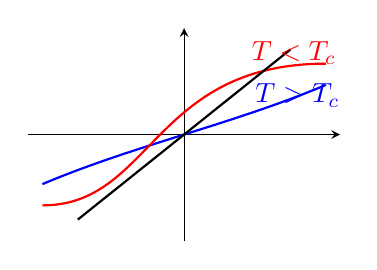
\begin{tikzpicture}[scale=0.9,>=stealth]
  \draw[->] (-2.2,0) -- (2.2,0);
  \draw[->] (0,-1.5) -- (0,1.5);
  \draw[blue,thick] (-2,-0.7) .. controls (-0.7,-0.15) and (0.7,0.15) .. (2,0.7);
  \draw[red,thick] (-2,-1.0) .. controls (-0.45,-1.0) and (-0.45,1.0) .. (2,1.0);
  \draw[black,thick] (-1.5,-1.2) -- (1.5,1.2);
  \node[blue] at (1.6,0.55) {$T>T_c$};
  \node[red] at (1.55,1.15) {$T<T_c$};
\end{tikzpicture}
\end{center}

\subsection{Curie--Weiss}

For $\beta\muB B\ll 1$: small $B$, high $T$, paramagnet.

\[
  \tanh x\sim x.
\]
\[
  \sigma
  =
  -\frac12
  \left(
  \beta\muB B-\frac12\beta Jz\sigma
  \right).
\]
Therefore
\[
  \sigma
  =
  \frac{-\frac12\beta\muB B}{1-\frac14\beta Jz}
  =
  \frac{-\frac12\muB B}{\kB\left(T-\frac{Jz}{4\kB}\right)}
  =
  \frac{-\frac14 g\muB B}{\kB(T-T_c)}.
\]

\[
  m=-g\muB\langle\sigma\rangle,
  \qquad
  M=-ng\muB\langle\sigma\rangle.
\]

\[
  \chi_{\mathrm{Curie\text{-}Weiss}}
  =
  \mu_0\frac{dM}{dB}
  =
  \frac{\mu_0\muB^2}{\kB T}\,
  \frac{1}{1-T_c/T}.
\]

For a ferromagnet:
\begin{center}
\begin{tikzpicture}[scale=0.9,>=stealth]
  \draw[->] (0,0) -- (3.2,0) node[right] {$T/T_c$};
  \draw[->] (0,0) -- (0,2.2) node[above] {$\sigma$};
  \draw[thick] (0,1.6) .. controls (1.1,1.6) and (2.4,0.9) .. (2.65,0);
  \node[below] at (2.65,0) {$1$};
\end{tikzpicture}
\end{center}

\subsection{Pauli Paramagnetism Near the Fermi Surface}

\[
  \varepsilon(\uparrow)
  =
  \frac{\hbar^2k^2}{2m}+\muB B,
  \qquad
  \varepsilon(\downarrow)
  =
  \frac{\hbar^2k^2}{2m}-\muB B.
\]

\[
  H_e=\frac{p^2}{2m}+g\muB\vect B\cdot\vect\sigma.
\]

\[
  M=-\frac{1}{V}\frac{dE}{dB}
  =
  -\frac{\muB}{V}\left(\#\uparrow-\#\downarrow\right).
\]

The relevant area near the Fermi level is
\[
  \text{Area}\sim \frac{g(\epsF)}{2}\,\muB B.
\]

Thus
\[
  \#\uparrow \text{ has } \frac{g(\epsF)}{2}\muB B \text{ less},
  \qquad
  \#\downarrow \text{ has } \frac{g(\epsF)}{2}\muB B \text{ more}.
\]

\[
  M=\frac{g(\epsF)\muB^2 B}{V}.
\]
\[
  \chi
  =
  \frac{\mu_0\muB^2g(\epsF)}{V}.
\]
Using
\[
  g(\epsF)=\frac{3N}{2\epsF},
\]
\[
  \chi
  =
  \mu_0\muB^2\frac{3N}{2\epsF}.
\]

\end{document}
